\chapter{Eztabaida.}

\section{Eguzki-sistemaren integraziorako egungo metodoak.}


Tesiaren sarreran azaldu genuenez, gure helburua eguzki-sistemaren epe luzeko eta doitasun handiko inplementazio eraginkorra proposatzea da. Atal honetan, egungo eguzki-sistemaren simulazioetan erabiltzen diren metodo eta inplementazioen laburpena egingo dugu. Bi eratako simulazioak aztertuko ditugu. Batetik, eguzki-sistemaren  efemerideak ditugu; eguzki-sistemaren eredu konplexuak eta epe tarte txikietarako (ehunka urtekoak) integrazioak konputatzen dituzte. Bestetik, astronomi arloaren inguruko ikerketetarako eguzki-sistemaren integrazio luzeak ditugu: eguzki-sistemaren eredu sinpleagoak eta milioika urteko integrazioak konputatzen dituzte. 

\subsection*{Efemerideak.}

Konputagailuen aurreko garaian, efemerideak teoria analitikoetan oinarritutako serie funtzioen bidez kalkulatzen ziren. Soluzio hauetan, Fourier-en serie trigonometriko luzeen ebaluazioa egin behar zen. $1960$ hamarkadan, eguzki-sistemaren ezagutza hobetu zenean (espazio bidaiak eta behatoki astronomikoen aurrerapenak medio), serie oso luzeak kalkulatu behar zituzten, eta orduan zenbakizko integrazioen bidezko soluzioak eraginkorragoak bilakatu ziren \cite{Kaplan2015}.   
   
Eguzki-sistemaren gorputzen efemeride modernoak, mugimenduaren ekuazio diferentzialen (\ref{eq:nbody}) zenbakizko integrazioaren bidez kalkulatzen dira. Integrazioaren hasierako balioak eta ereduaren parametroak, sateliteen bidez jasotako datuekin kontrastatu egiten dira.

Efemerideak, \emph{Chebyshev} polinomio moduan adierazten dira. Integrazio tarteak, $2.000.$ urte inguruko ehunka urtekoak izaten dira. Zenbakizko integrazio hauetan, biribiltze errorea gai garrantzitsua da. $128$-biteko aritmetikaren aukera baztertzen da, konputazioa oso garestia delako eta $64$-biteko doitasuneko aritmetika hobetzen dituzten teknika konputazionalki merkeagoak, aplikatzen dira. 

Efemerideetarako, eguzki-sistemaren eredu konplexua aplikatzen da. Gorputz nagusien arteko indar grabitazionalez gain, erlatibitate efektua, asteroideek eragindako grabitazio indarrak, gorputzen formen eragina eta beste hainbat indar ez grabitazionalak kontutan hartzen dituzte. Mugimenduaren ekuazio diferentzialak, era honetakoak izaten dira \cite{Feinga2015},      
      \begin{equation*}
      \ddot{x}_{Planet}= \sum_{A \neq B} \mu_B \frac{r_{AB}}{\|r_{AB}\|^3}+\ddot{x}_{GR} (\beta,\gamma,c^{-4})+ \ddot{x}_{AST,300}+ \ddot{x}_{J_2}.
      \end{equation*}

Hauek dira, ekuazio hauen konplexutasuna erakusten duten ezaugarri batzuk:      
      \begin{itemize}
      \item Gorputz kopurua: $8$ planetak, ilargia, Pluton eta 300 asteroide.
      \item Erlatibitate efektua (GR): Einstein-Imfeld-Hoffmann, $c^{-4}$ PPN hurbilketa.
      \item $J_2$: eguzkia esferikoa ez izatearen eragina. 
      \item Urrats luzera, $h=0.055$ egunekoa da.
      \end{itemize}   

\subsubsection*{Erlatibitate efektua.}
Eguzkiaren erlatibitate efektua kontutan hartzen duten ekuazio diferentzialak azalduko ditugu \cite{Kopeikin2011}.
\begin{equation}
\dot{q_i}=v_i, \  i=0,1,\dots N
\end{equation}
\begin{multline} 
\dot{v_i}= \sum_{j=0,j \neq i}^{N} \frac{Gm_j}{\|q_j-q_i\|^3} (q_j-q_i)
           \bigg(1- \frac{2(\beta+\gamma)}{c^2} \sum\limits_{k=0, k \neq i}^{N} \frac{Gm_k}{\|q_k-q_i\|} 
                  - \frac{2\beta-1}{c^2}        \sum\limits_{k=0, k \neq j}^{N} \frac{Gm_k}{\|q_k-q_j\|} \\
                  + \gamma \big(\frac{v_i}{c}\big)^2 + (1+\gamma) \big(\frac{v_j}{c} \big)^2 
                  - \frac{2(1+\gamma)}{c^2} v_i \ v_j \\
                  - \frac{3}{2c^2} \big(\frac{(q_i-q_j) v_j}{\|q_j-q_i\|} \big)^2+                  
                  \frac{1}{2c^2}(q_j-q_i) \dot{v_i} \bigg) \\
           + \frac{1}{c^2} \sum_{j=0,j \neq i}^{N} \frac{Gm_j}{\|q_j-q_i\|^3} 
             ((q_i-q_l) ((2+2\gamma)v_i-(1+2\gamma)v_j)) (v_i-v_j) \\
           + \frac{3+4\gamma}{2c^2} \sum_{j=0,j \neq i}^{N} \frac{Gm_j \dot{v_j}}{\|q_j-q_i\|}                                      
\end{multline}

\begin{table}[h]
\caption{Konstanteak}
\label{tab:1}       % Give a unique label
\centering
\begin{tabular}{l l l }
\hline
  c             &  $299792.458$ km/s           & Argiaren abiadura  \\
%\hline
  au            &  $149597870.700$ km          & Unitate Astronomikoa  \\
%\hline 	       
$\beta$          & $1.0$                       & PPN parametroa     \\
%\hline 
$\gamma$         & $1.0$                       & PPN parametroa     \\
\hline
\end{tabular}
\end{table}

\subsubsection*{Asteriodeak.}
Asteroideek, bereziki Marte planetaren mugimenduarengan eragina dute (\ref{fig:asteroideak} irudia) eta kontutan hartzekoak, barne-planeten mugimenduaren doitasun handiko emaitzak behar ditugunean . Bost asteroide nagusiren masak (Ceres, Pallas, Vesta, Iris eta Bamberga) Merkurio eta Pluton planeten mailakoak direnez, integrazioetan gehitzen dira. Asteroide txikien talde handia, estimazioen bidez simulatzen dira.

\begin{figure} [h]
\centerline{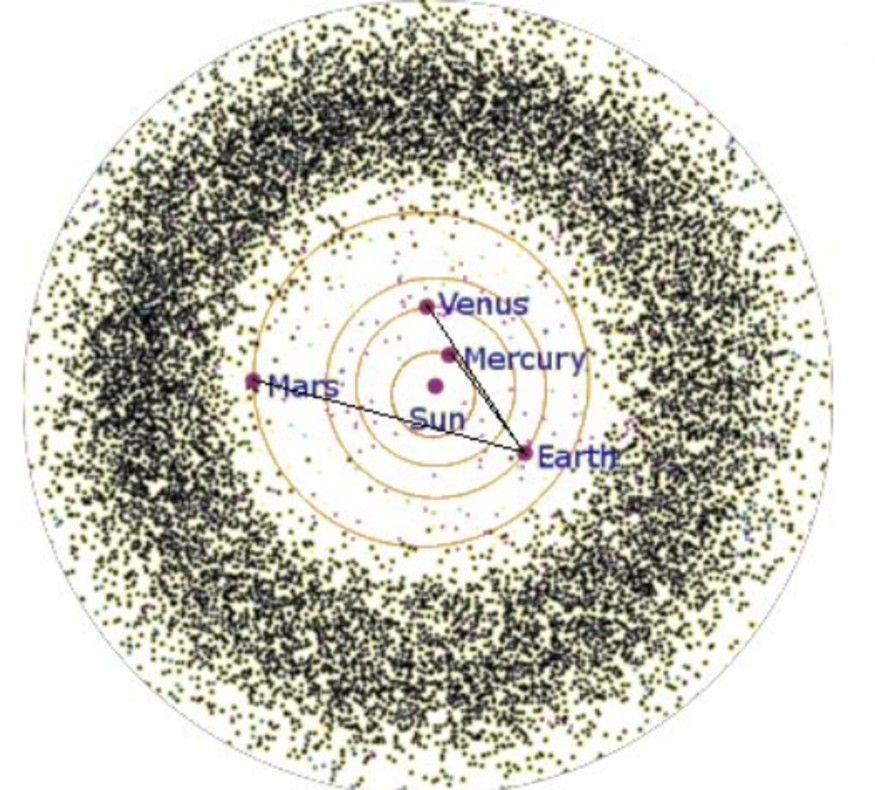
\includegraphics [width=6cm, height=4cm] {Asteroideak}}
\caption{Asteroideak.}
\label{fig:asteroideak}
\end{figure} 

  
\subsubsection*{Hiru efemerideak.}

Gaur-egun, eguzki-sistemaren planeten hiru efemeride kalkulatzen dira.
\begin{enumerate}
\item Jet Propulsion Laboratory (\emph{EEBB}) \emph{NASA}-ko erakundeak DE (Development Ephemerides) izeneko efemerideak konputatzen dituzte.

      $1984$. urtean kalkulatu zen lehen efemeridea (DE-200) eta $2.014$. urteko \emph{DE-430} \cite{Folkner2014} efemeridea da, publikatutako azken efemeridea. Azken efemeride honen integrazio tartea, $1550-2650$ urtetakoa izan da.

      Zenbakizko integrazio metodoa, urrats luzera eta  ordena aldakorreko \emph{Multistep Adams} metodoa \cite{Krogh1997} (\emph{DIVA}/\emph{QIVA}) da. \emph{QIVA} doitasun laukoitzeko ($128$-bit) bertsioari deitzen zaio: mugimenduaren ekuazioen Newton zatia, doitasun laukoitzean kalkulatzen da eta ekuazioaren gainontzeko zatia, doitasun bikoitzean.

\item Institut de Méchanique Céleste et de Calcul des Ephémérides (IMCCE,Paris Observatory) INPOP (Intégrateur Númerique Planétaire de l'Observatoire de Paris) izeneko efemerideak.
      
      $2.000$. urte arte, efemerideak kalkulatzeko teori analitikoetan oinarritu ziren. $2.003$. urtean, zenbakizko integrazioaren bidezko lehen efemeridea kalkulatu zuten eta \emph{INPOP13c}  \cite[$2.014$]{Fienga2008} publikatutako azkena da.
           
	  Zenbakizko integrazio metodoa: $12$ ordeneko \emph{Adams-Cowell} metodoa da eta urrats finkoa aplikatzen dute.
	  
	  Doitasuna: C lengoaian inplementatuta dago eta \emph{Intel} makinetako $80$-biteko doitasuna erabiltzen du. Era berean, modu merkean  doitasun laukoitza simulatuz, urrats zuzentzaile (corrector step) bat aplikatzen dute \cite{Fienga2008}.  
	  
  
\item Institute of Applied Astronomy (\emph{IAA}, St. Petersburg), EPM (Ephemerides Planets-Moon) izeneko efemerideak.
      
      $1.980$. urtetik aurrera, zenbakizko integrazioen bidezko efemerideak kalkulatu dituzte eta  \emph{EPM2.013}  \cite[2.014]{Pitjeva2014} publikatutako azken efemeridea da.
      
      Zenbakizko integrazio metodoa, \emph{Everhart} izeneko \emph{IRK} metodoa (Gauss-Radau) da. $23$ ordeneko metodoa eta urrats luzera finkoa aplikatzen dute.
            
      Doitasuna. Inplementazioak (software package ERA), \emph{Intel} makinetako $80$-biteko doitasuna erabiltzen dute.
      
\end{enumerate}


%\ref{fig:668} taulan, planeten efemerideen doitasunaren eboluzioa ikus daiteke. Hiru efemerideak antzeko doitasuna azaltzen dutela gehitu beharra dago. 
%\begin{figure} [h]
%\centerline{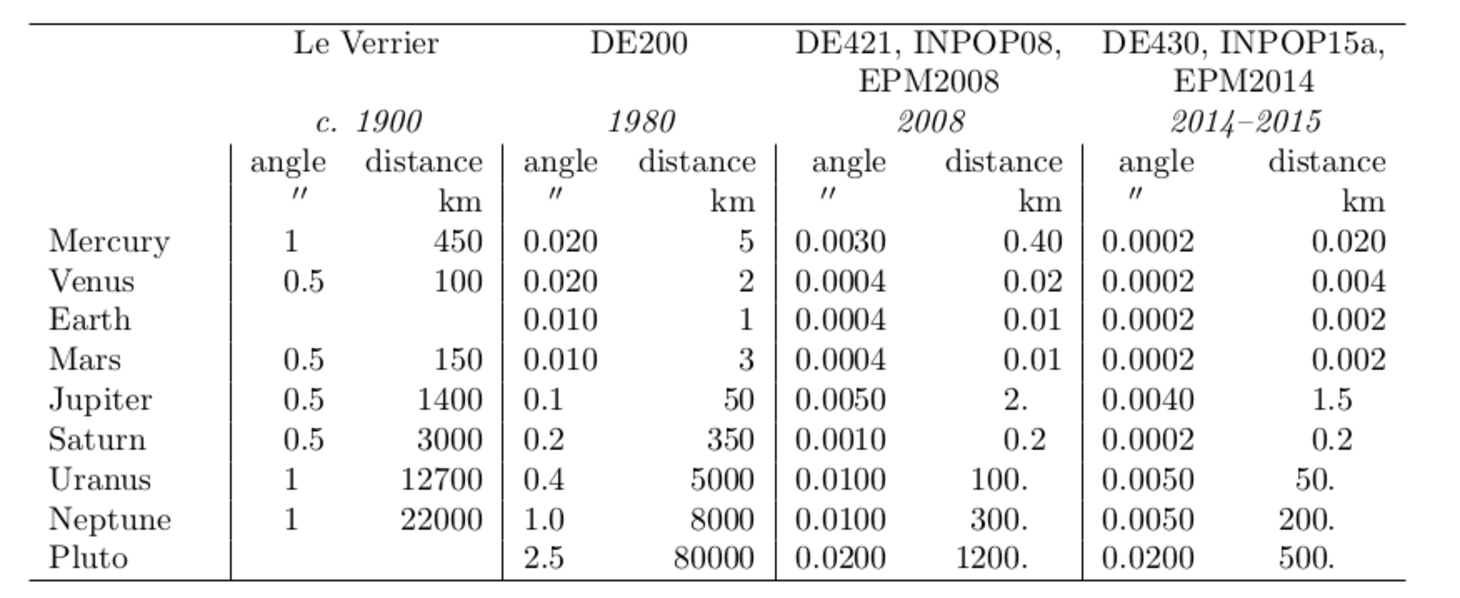
\includegraphics [width=10cm, height=6cm] {Efemerideak}}
%\caption{Efemerideen doitasunaren eboluzioa.}
%\label{fig:668}
%\end{figure} 
%

\subsection*{Eguzki-sistemaren integrazio luzeak.} 


A.Morbidellik \cite{Morbidelli2002} eguzki-sistemaren zenbakizko integrazioen algoritmoen garapenaren azterketan, garai hauek bereizten ditu:
\begin{enumerate}

\item Garai klasikoa.

$90$. hamarkada hasiera arte, urrats luzera aldakorreko integratzaileak erabiltzen dira: Runge-Kutta (Dormand et al. $1987$), Bulirsch and Stoer ($1966$), Radau (Everharht, $1985$), eta Störmer ($1990$). Garai honetan integrazio tarteak, $10^4-10^6$ urte artekoak dira.  

\item Garai sinplektikoa.

Wisdom eta Holman-en \cite[1991]{Sussman1992} lanarekin, eguzki-sistemaren azterketarako integratzaile sinpletikoen erabilera zabaldu zen. Garai honetan, ($10^8-10^9$) urte arteko eguzki-sistemaren integrazioak egin ziren.  

\item Garai estatistikoa.

Planeten eta gorputz txikien (asteroide, meteoritoak) arteko kolisio gertuko egoerak kalkulatzen dituzten algoritmoak garatu ziren. Inplementazio berri hauetan, milaka gorputzen integrazio azkarra egin daiteke. Horrela, asteroide eta meteoritoen orbiten distribuzio azterketa estatistikoak egin ziren.

\item Planeten sorrera garaiko azterketak.

Eguzki-sistemaren sorrerari buruzko simulazioak nagusituko dira; masa handiko gorputzen arteko kolisio gertuko egoerak gertatzen diren integrazioak konputatzen dira. 
 
\end{enumerate}

Eguzki-sistemaren integrazioetarako nagusiki, bi integratzaile famili aplikatzen dira: 
\begin{enumerate}
\item Integratzaile simetrikoak.

Metodo simetrikoen artean nagusiena, 4 ordenako \emph{Hermite} \cite{Aarseth2008} integratzailea da.
Urrats luzera tamaina aldakorreko integratzaile da, modu errazean inplementatu daiteke.  Hermite integratzailea konputazionalki garestia da eta bereziki, gorputz kopuru handia dituzten eta kolisio gertuko egoerak maiz gertatzen diren problemetan (eguzki-sistemaren sorrera, \dots) aplikatzen da.  

\item Sinplektikoak.

Gaur-egun, eguzki-sistemaren epe luzeko integrazioetarako, integratzaile sinplektikoak nagusitu dira. 

\end{enumerate}


\subsubsection*{Eguzki-sistemari egokitutako integratzaile sinplektikoak.}

Wisdom-ek eta Holman-ek \cite[1991]{Sussman1992}, eguzki-sistemaren epe luzeko simulazioetarako integratzaile  sinplektikoak (\emph{WH}) arrakasta izan zuen. Eguzki-sistema, mugimendu perturbatua duen sistema dinamikoa da eta ezaugarri honi egokitutako integratzaile eraginkorra garatu zuten. Jacobi koordenatuak  aplikatuz, N-gorputzen problemaren Hamiltondarra, bi zatitan banatu zuten,
\begin{equation*}
H(q,p)=H_K(p)+H_I(q) \ \ \ , \ \ H_K\gg H_I,
\end{equation*}
non $H_K$, Hamiltondar Kepleriarra (planeten eguzkiarekiko mugimendu kleperiarra) eta $H_I$, interakzioen Hamiltondarra (planeten arteko grabitazio interakzioak) diren. Integrazioaren urrats bakoitzean , Hamiltondar bakoitzaren soluzioa tartekatuz, problema osoaren ebazpena kalkulatzen da.  

\emph{WH} integratzailea, ondorengo metodo askoren aurrekaria kontsideratu bada ere, bere aplikagarritasuna mugatua da. Batetik, izar anitzeko planeten sistemak edo planeta-ilargiak sistemak integratzeko ez da egokia. Bestetik, \emph{WH} metodo sinplektikoa denez, urrats luzera finkoa aplikatu behar da eta hau, gorputzen arteko kolisiotik gertuko egoerak dituzten problemak modu eraginkorrean integratzeko eragozpen bat da. Arazo hauek gainditzeko, urteetan zehar algoritmo honen aldaerak proposatu dira eta jarraian, nagusienak aipatuko ditugu. 

Levinson eta Duncan-ek \cite[1994]{Levison1994}, \emph{WH} inplementazioa, integratzaile ez sinplektiko batekin konbinatu zuten, kolisiotik gertuko egoeren kalkulua hobetzeko. \emph{SWIFT} paketean, \emph{RMVS3} izeneko integratzailea inplementatu zuten. Duncan, Levinson eta Lee-k \cite[1998]{Duncan1998}, koordenatu heliozentrikoak erabiliz, Hamiltondarra beste modu honetan banatu zuten,  
\begin{equation*}
H(q,p)=H_K(p)+(H_C(p)+H_I(q))
\end{equation*}
eta kolisiotik gertuko egoerei, urratsa luzera txikituz aurre egin zioten. Inplementazio honek, \emph{SYMBA} izena du. Chambers-ek \cite{Chambers1999} koordenatu heliozentrikoetan oinarritu zen eta kolisiotik gertuko egoerak gertatzen diren uneetan, beste integratzaile  (Bulirsch-Stoer metodoa) batekin konbinatuz integratzen du. Inplementazio honek, \emph{MERCURY} izena du. Levinson eta Duncan-ek ($2000$), aurreko inplementazioaren arazo batzuk konponduz, \emph{Modified SYMBA} izeneko garapen berria burutu zuten.
Kvaerno eta Leimkuhler \cite{Kvaerno2000} eta beste autore batzuk ere, antzeko ideiak landu dituzte.

Wisdom eta Holmanek proposatutko Hamiltondarraren banaketa, (\ref{eq:stverlet})~\emph{Leapfrog} metodoaren bidez integratzen da eta beraz, 2 ordeneko da. Orden altuagoko ($p>2$) metodoak definitzeko, koefiziente negatiboak erabili behar zela uste zen \cite{Yoshida1993,Laskar2001} eta orduan ez dira interesgarriak, \emph{Leapfrog} metodoak eraginkorragoak baitira. 

%\paragraph*{Adibidea.}
%Yoshidaren $p=4$ ordenako metodoa. $\phi_h$ oinarrizko metodoa \emph{Leapfrog} izanik, metodoaren konposaketari dagokion 4 ordeneko konposizio metodoa, era honetan definitzen da,
%\begin{equation*}
%\Psi_h=\phi_{\gamma_1 h} \circ \phi_{\gamma_0 h} \circ \phi_{\gamma_{1 h}},
%\end{equation*}  
%non  $\gamma_0=-2^{1/3}/(2-2^{1/3})$ eta $\gamma_1=1/(2-2^{1/3})$.

Beranduago, McLachlan-ek \cite[1995]{McLachlan1995} eta Laskar-ek  \cite[2001]{Laskar2001} koefiziente negatiboen arazoa gainditu zuten eta koefiziente positiboekin definitutako ordena altuko Splitting eskemak aurkitu zituzten. Berriki, Blanes-ek \cite[2012]{Blanes2013} ordena altuko Splitting eskema berriak eta eraginkorrak aurkitu ditu. 

Hernandez eta Bertschinger-ek \cite[2015]{Hernandez2015} N-gorputzen problema grabitazional eta kolisiodunetarako $2$ ordenako integratzaile sinplektiko berri bat proposatu dute. Hernandez eta Bertschinger-ek \cite{Hernandez2015} koordenatu kartesiarretan oinarrituz, N-gorputzen problema, 2-gorputzen azpiproblemetan banatzen dute.

% eta honako Hamiltondarraren banaketa proposatzen dute,
%\begin{align}
%\begin{split}
%&H=T+V, \\
%&H=T+ \sum_{i} \sum_{i>j} V_{ij}, \\
%&H=T+ \sum_{i} \sum_{i>j} (K_{ij}-T{ij})
%\end{split}
%\end{align}

\subsection*{Splitting metodoak.}

Splitting metodoak, era honetako perturbatutako Hamiltondar sistemak,
\begin{equation}
\label{eq:Hban}
H=H_A+\epsilon H_B,
\end{equation}
integratzeko aplika daitezke, non $H_A$ eta $H_B$ independenteki integragarriak diren. Pentsatzeko da, eguzki-sistemaren eredu errealistetan hainbat indar ez grabitazionalak modu honetan gehitzeko, zailtasunak izan ditzakegula.  

Laskar-ek \cite[2011]{Laskar2011}, epe luzeko zenbakizko integraziorako  $1/c^2$ ordenako eguzkiaren erlatibitate efektua   kontsideratu zuen. Horretarako, Saha eta Tremain-ek \cite{Saha1994} finkatutako teknikan oinarritzen da. Teknika honetan, (\ref{eq:Hban}) Hamiltondar banagarriei egokitzen zaien erlatibitate efektuaren espresioa lortu zuten eta gainera modu eraginkorrean kalkulatu daiteke. Kontutan hartuko bagenitu, bi planeta handienen (Jupiter eta Saturno) erlatibitate efektua, ekuazioak ez dira gehiegi konplikatzen eta errorea txikiagoa lortuko genuke. Splitting metodoetan ez da posible erlatibitate efektu hauek gehitzea eta horregatik, ez direla kontutan hartzen. 
 
Eguzki-sistemaren integrazioetarako, (\ref{eq:Hban}) Hamitondarraren banaketa, Jacobi koordenatuak edo heliozentrikoak aplikatuz lortzen da.
Koordenatu cartesiarrak, ezin daitezke erabili.

Muga hauek ez ditugu, IRK metodoak aplikatzeko. Ekuazio diferentzial orokorrei aplika daitekeenez, askatasun osoa dugu behar diren ekuazioak gehitzeko eta interesatzen zaigun koordenatu sistema aplikatzeko.  
 

\section{Hasierako inplementazioa: ereduen deskonposaketa.}


Hasierako planteamendu honetan,  Newton sinplifikatua aplikatzen dugu eta  sistema lineala LU deskonposaketaren bidez askatu ordez, puntu-finkoaren bidez askatzen dugu.

Ekuazio diferentzialak $\dot{y}=f(y)$ era honetan deskonposatzen ditugu,
\begin{align*}
&\dot{y}=\tilde{f}(y),\\
&g(y)=f(y)-\tilde{f}(y).
\end{align*}

Honako sistema lineala askatzeko,
\begin{align*}
Y_i^{[k+1,l]}=y_0+ h \sum a_{ij} \big( \tilde{f}(Y_i^{[k,l]})+g(Y_i^{[k,l-1]})),
\end{align*}
puntu-finkoaren iterazioa aplikatzen dugu.

Planteamendu honetan, IRK-Newton inplementazioarekiko hiru desabantaila aurkitu ditugu: 
\begin{enumerate}
\item Barne kalkuluen doitasuna. 

IRK-Newton sinplifikatuaren inplementazioan, eragiketa konplexuenak doitasun txikiagoan kalkula daitezke. Hasierako inplementazio honetan, barne iterazioak inplementazioaren doitasunean kalkulatu behar dira.

\item Jacobiarra.

IRK-Newton sinplifikatuan, Jacobiarra urrats bakoitzean behin kalkulatu behar da. Hasierako inplementazioan, Jacobiarra ()iterazio bakoitzean  aldatu egiten da (kostu handiagoa).
\item Ereduen hiru maila erabiltzen da.\\
$k+g$ deskonposaketan $g=f(u)-\tilde{f}(u)$ ez da hain sinplea. 
\end{enumerate}

\begin{align*}
&M*\triangle L=R,
&\triangle L=R-(M-I) \triangle L
\end{align*}
non $M-I=(h*BAB^{-1}\otimes J)$ den. Puntu finkoa aplikatzen genuen $M-I=0$ hartuz.

\subsubsection*{ideiak1}
Sistema dinamikoa, sistema sinplifikatuaren perturbazioa kontsideratuko dugu.  
 We consider the dynamical motion as a perturbation of a simplified dynamical system.  We will use a perturbed initial value problem (IVP) form,
 \begin{align*}
 \dot f(y)=  k(y) + \epsilon g (y), \ \ g\ll k.   
 \end{align*}
 where $k(y)$ is simplified dynamical system, and the evaluation cost is low and
$g(y)$ is complex dynamical system  and  the evaluation cost is high. We propose an algorithm that reduces the number of evaluations of complex part  and so, reduce the cpu time. 


We have presented a new iterative solution for a Hamiltonian system \cite{Makazaga2015a}. We have splitted the function in a expensive function ($g$) and a cheap function ($k$) evaluation. We will consider an initial value problem where $g()$ is the perturbing function with $\epsilon<<1$.
\begin{equation} \label{eq:2}
{\dot{u}}=f(u)= k(u)+g(u).  \ \ \ \ \ \ \ \ \ u(t_0)=u_0
\end{equation}
where $k,g: \ {{\Re}}^{6N} \ \longrightarrow {{\Re}}^{6N}.$

\vspace{5mm}
We have proposed the next iterative solution \cite{Makazaga2015a}.\newline

\begin{algorithm}[H]
\For{k=1,2,...}{
\BlankLine
${{Y_i}^{[k]}=y_n+h\ \ \sum^s_{j=1}{a_{ij}(\ k({Y_j}^{[k]})+g({Y_j}^{[k-1]})) }}$; 

\BlankLine
}
\end{algorithm}

We can interprete the new iteration method as a Simplified Newton method, when we use the Jacobian of the $k()$ function such as approximation.

\subsubsection*{meta-algoritmoa}

We propose the next algorithm for initial value problem of the form (~\ref{eq:2})

\vspace{5mm} %5mm vertical space
\begin{algorithm}[H]

 \For{$n\leftarrow 1$ \KwTo $endstep$}{
  \BlankLine
  Initialization\ $Y^{[0]}_i, W^{[0]}_i\ i=1,\dots\,s$\;
  k=1\;
  Solve \ ${Y_i}^{[k]}=y_n+h\  \sum^s_{j=1}{a_{ij}\ k({Y_j}^{[k]})+W^{[k-1]}_i\ \ \ }$\;
  \BlankLine
  \While{not coverge}{
     \BlankLine
     k++\;
     $W^{[k-1]}_i= h\ \sum^s_{j=1}{a_{ij}\ g({Y_j}^{[k-1]})}$\; 
     Solve \ ${Y_i}^{[k]}=y_n+h\  \sum^s_{j=1}{a_{ij}\ k({Y_j}^{[k]})+W^{[k-1]}_i\ \ \ }$\;
     \BlankLine
  }  
  $y_{n+1}=y_n+h\ \sum^s_{j=1}{b_{i}\ f({Y_j}^{[k]}) \ }$\;
  \BlankLine
 }
 \caption{Meta-Algorithm}
\end{algorithm}


\subsubsection*{Advantages.}

The main advantage of the new algorithm  is its flexibility. We can solve problems in differents ways, and taking all good properties of the Runge-Kutta inplicit method. Next We will explain some:       
\begin{itemize}
  \item Iteration method.\\
  Barne iterazioan, metodo egokiena aplikatu daiteke. Problema ez-stiffa bada, puntu finkoaren bidez askatu daiteke eta problema stiffa bada Newton sinplifikatuaren bidez.
 
  \item Problema independenteak.\\
Era honetako deskonposaketa bat dugunean,

\begin{align*}
f\left ( \begin{array}{c}
   y_1 \\
   y_2 \\
\end{array} \right)=
\left ( \begin{array}{c}
   k_1(y_1) \\
   k_2(y_2) \\
\end{array} \right)+
\left ( \begin{array}{c}
   g_1(y_1,y_2) \\
   g_2(y_1,y_2) \\
\end{array} \right),
\end{align*}

eredu sinplifikatua problema independenteak osatzen dituzte eta barne iterazioak modu independentean kalkula daitezke. N-gorputzen eguzki-sistemaren adibidean, eredu sinplifikatua $k(y)$ (eguzkiarekiko interakzioa) planeta bakoitzarentzat problema independentea dugu. Kasu honetan urrats bat finkatuta, kanpo planeten $k(y)$ problema barruko planeta baino azkarrago konbergituko du. 
\end{itemize}  

\subsubsection*{Inner iterations.}


We know that we can use any method to solve inner nonlinear system. We implement the algorithm using the fixed-point iteration for the inner nonlinear system,

\vspace{5mm} %5mm vertical space
 Solve \ ${Y_i}^{[k]}=y_n+h\  \sum^s_{j=1}{a_{ij}\ k\left({Y_j}^{[k]}\right)+W^{[k-1]}_i\ \ \ }$\;
 
\begin{algorithm}[H]
 \BlankLine
  $l=0$\;
  $Y_{n,i}^{[k,0]}=Y_{n,i}^{[k-1]}$\;
  \While{ (konbergentzia lortu)}
  {
   \BlankLine
   $l=l+1$\;  
   \BlankLine
   $K_{n,i}^{[k,l]}=k(Y_{n,i}^{[k,l-1]})$\;
   $Y_{n,i}^{[k,l]}=y_{n} + h \sum\limits_{j=1}^{s} \ a_{ij} \ K_{n,j}^{[k,l]}  +  W_{n,i}^{[k-1]} $\;
  }
 \caption{Barne iterazioa: puntu-finkoa}
\end{algorithm}

\subsubsection*{Orokorpena.}

Aurreko atalean, maila bakarreko ereduen deskonposaketa aztertu dugu. Ideia orokortuz, eredu deskonposaketa maila ezberdinetan egin daiteke. Problema bat emanda $\dot{y} =f(y)$, 

\begin{align}
\mbox{1. maila} \ \
\left \{ \begin{array}{c}
  \mbox{Eredu osoa.   } f(y) \\[.25cm]
  \mbox{Eredu sinplea.    } \tilde{f}(y)  \\
\end{array} \right.
\ \Rightarrow \ \
f =\tilde{f}+(f-\tilde{f})  
\end{align}

\begin{align}
\mbox{2. maila} \ \
\left \{ \begin{array}{c}
  \mbox{Eredu osoa.   }\tilde{f}(y) \\[.25cm]
  \mbox{Eredu sinplea.    }\tilde{\tilde{f}}(y)  \\
\end{array} \right.
\ \Rightarrow \ \
\tilde{f} =\tilde{\tilde{f}}+({\tilde{f}}-\tilde{\tilde{f}})  
\end{align}

\paragraph*{Adibidea.}
Eguzki-sistemaren eredu konplexuago ditugunean, meta-algoritmoa modu errekurtsiboan aplika daiteke. Adibide moduan, demagun eguzki-sistemaren problemaren ekuazio diferentzial hauek ditugula,
\begin{equation*}
\dot{y}=f(y), \ f(y)=k(y)+g(y)+r(y),
\end{equation*}
non
\begin{align*}
&k(y): \ \text{kepleriarra.}\\
&g(y): \ \text{planeten arteko grabitazio interakzioak.}\\
&r(y): \ \text{egukiarekiko eralatibitate efektua.}
\end{align*}

Meta-algoritmoa errekurtsiboki modu honetan aplikatuko genuke,
\begin{align*}
{{Y_i}^{[k]}=y_n+h\ \ \sum^s_{j=1}{a_{ij}(\ k({Y_j}^{[k]})+g({Y_j}^{[k-1]}))+r({Y_j}^{[k-1]}) }}\\
{{Y_i}^{[k,l]}=y_n+h\ \ \sum^s_{j=1}{a_{ij}(\ k({Y_j}^{[k,l]})+g({Y_j}^{[k-1,l]})+r({Y_j}^{[k-1],l-1})) }}
\end{align*}

\subsubsection*{Adierazpena.}

Ekuazio diferentzialen deskonposaketak, zuhaitz moduan adieraz daitezke.

\begin{equation*}
\dot{y}=f(y).
\end{equation*}


\begin{tikzpicture}[scale=.8]
%\draw (-1,-2) grid (5,2);
\filldraw[black] (0,0) circle (2pt);
\end{tikzpicture}

\begin{equation*}
f\left ( \begin{array}{c}
   y_1 \\
   y_2 \\
\end{array} \right)=
\left ( \begin{array}{c}
   f_1(y_1) \\
   f_2(y_2) \\
\end{array} \right)+
\left ( \begin{array}{c}
   g(y) \\
\end{array} \right),
\end{equation*}

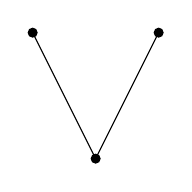
\begin{tikzpicture}[scale=.8]
%\draw (-1,-2) grid (5,2);
\filldraw[black] (0,0) circle (2pt);
\filldraw[black] (1,2) circle (2pt);
\filldraw[black] (-1,2) circle (2pt);
\draw (0,0) -- (1,2);
\draw (0,0) -- (-1,2);
\end{tikzpicture}

\begin{equation*}
f_1\left ( \begin{array}{c}
   y_1 \\
\end{array} \right)=
\left ( \begin{array}{c}
   f_{11}(y_{11}) \\
   f_{12}(y_{11},y_{12}) \\
   f_{13}(y_{11},y_{12},y_{13}) \\
\end{array} \right)+
\left ( \begin{array}{c}
   g_1(y_1) \\
\end{array} \right),
\end{equation*}


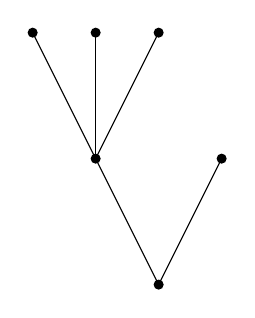
\begin{tikzpicture}[scale=.8]
%\draw (-1,-2) grid (5,2);
\filldraw[black] (0,0) circle (2pt);
\filldraw[black] (1,2) circle (2pt);
\filldraw[black] (-1,2) circle (2pt);
\filldraw[black] (-2,4) circle (2pt);
\filldraw[black] (-1,4) circle (2pt);
\filldraw[black] (0,4) circle (2pt);
\draw (0,0) -- (1,2);
\draw (0,0) -- (-1,2);
\draw (-1,2) -- (-2,4);
\draw (-1,2) -- (-1,4);
\draw (-1,2) -- (0,4);
\end{tikzpicture}

\subsubsection*{Adaptative tol}
We use outer's same stop criterion for the inner iteration except the tolerance. We use a fixed tolerance for outer iteration and adaptative tolerance for the inner ieration.

We have splitted the function in a expensive function ($g$) and a cheap function ($k$) evaluation. Our goal is to get tolerance with the minimum CPU time. We want to run each step with the minimum outer iterations (expensive) and with the only necessary inner iterations (cheap). 

So, we define a adaptative tol to execute only necesary and sufficient inner iterations for each outer iteration. We have to take into account that we need two inner iterations to determine the inner iteration tolerance.\\

\subsubsection*{N-Body problem.}

We will use Newtonian model of the Solar System for our test problems. The simplified part of the system is the keplerian and the perturbation, is the interactions between planets.

\[H\left(q,p\right)=H_k+H_I,\ \ \ \ H_k\ll \ H_I\] 
\begin{equation}
H_k(q,p)=\frac{1}{2}\ \sum^N_{i=0}{\frac{{p_i}^2}{m_i}}-\ \ Gm_0\sum^N_{i=1}{\frac{m_i}{\left\|q_i-q_0\right\|}}\  
\label{eq:h1}
\end{equation}

\begin{equation}
H_I(q)=\sum^N_{1\le i<j\le N}{\ \frac{G\ m_im_j}{\left\|q_j-q_i\right\|}}\   
\label{eq:h2}
\end{equation}

And the corresponding differential equations could be calculated
\begin{equation}
\dot{q}={\nabla }_pH(q,p)\ \ \, \ \ \dot{p}=-{\nabla }_qH(q,p)
\end{equation}

\subsubsection*{Strength and limitations.}
\label{sec:43}

\vspace{5mm}
\textit{Close approaches.}\\
Our new algorithm do not handle close approaches and collisions.  Reference to regularization ?
Why is important? It could not be possible to calculate an accurate solution for the orbital motion of the Earth over more than 100 Myr because the Solar System is chaotic.  In recent article Laskar \cite{Laskar2011a} show that largest bodies in the asteroid belt, Ceres, Pallas and Vesta limited more the precise solution about 60 Myr. Among these asteroides happen close encounters and this strong interactions during close encounters also affect the planetary motions. 


\vspace{5mm}
\textit{Exoplanets.}\\
These approximations are appropiate for applications in the Solar System, but more general methods are needed to describe a variety of explanetary systems.  They require dynamical theories that describe more extreme motions than those of the relatively placid planetary orbits of the Solar System. Fabrycky \cite{Fabrycky2010}

\section{IRK puntu-finkoa: oinarriak.}

\subsection*{Atalen hasieraketa.}

Puntu-finkoaren iterazioan, atalen hasieraketa teknika ezberdinak ikertu ditugu. 
\begin{enumerate}
\item Metodo esplizituak.

Euler-en eta Euler-hobetuaren metodoak aztertu ditugu.

\item Kepler fluxua.

Eguzki-sistema, perturbatutako sistema Kepleriarra dela jakinda, atalak Kepler fluxuaren bidez hasieratu daitezke.

\item Interpolazio polinomioak.

Aurreko urratseko ataletako informazioa erabiliz, urrats berriaren atalen hasieraketa lortzen dugu. Problema zurruna ez denean interesgarria da. 

Bide honetatik, teknika aurreratuagoak ere aztertu ditugu (maila txikiko polinomioen bidezko hasieraketak). Era berean, B-Serieak \cite{Chartier2010} teknikan oinarrituz, interpolazio estandarra \cite{Laburta1998} hobetzeko saiakera egin dugu baina ez dugu hau hobetzea lortu. Metodo estandarrarekin, urrutien dagoen ataletarako hasieraketa txarra lortzen da eta atal askotako metodoentzat, arazo hau, eragozpen handia izan daiteke.  

\end{enumerate}

\subsection*{Geratze irizpidea.}


\subsubsection*{Norma.}
Lehengo, geratze irizpidea definitzeko norma zalantzan jarri dugu. Hairer-ek, geratze irizpidean aplikatzen duen norma hauxe da,
\begin{equation*}
\Delta Y= \max_{i=1,\dots,s} \|Y_i^{[k]}-Y_i^{[k-1]}\|_{\infty}.
\end{equation*}

Aukera ezberdinak aztertu ditugu,
\begin{enumerate}
\item Lehen bertsioa.

\begin{align*}
\Delta Y= \max_{1 \leqslant j \leqslant s} \frac{\max_{1 \leqslant j \leqslant s} |\Delta Y_i^j|}
                                                {(\max_{1 \leqslant j \leqslant s}|Y_i^j|)+\delta},
\end{align*}
non $\delta \approx 10^{-20}$ zero den kasua ekiditeko balio txikia den eta $y=(y^1,\dots,y^d)$.

\item Bigarren bertsioa.

Each user can define her own norm. We define specific norm for the N-body problem.
We define a set of internal stages $Y$ for the new approximation and $\tilde Y$ for the previous value.

\[Y=\left( \begin{array}{cccccc}
Q^{[1]}_1 & \dots  & Q^{[n]}_1 & V^{[1]}_1 & \dots  & V^{[n]}_1 \\ 
Q^{[1]}_2 & \dots  & Q^{[n]}_2 & V^{[1]}_2 & \dots  & V^{[n]}_2 \\ 
\dots  & \dots  & \dots  & \dots  & \dots  & \dots  \\ 
Q^{[1]}_s & \dots  & Q^{[n]}_s & V^{[1]}_s & \dots  & V^{[n]}_s \end{array}
\right)\ \  
\tilde Y=\left( \begin{array}{cccccc}
\tilde Q^{[1]}_1 & \dots  & \tilde Q^{[n]}_1 & \tilde V^{[1]}_1 & \dots  & \tilde V^{[n]}_1 \\ 
\tilde Q^{[1]}_2 & \dots  & \tilde Q^{[n]}_2 & \tilde V^{[1]}_2 & \dots  & \tilde V^{[n]}_2 \\ 
\dots  & \dots  & \dots  & \dots  & \dots  & \dots  \\ 
\tilde Q^{[1]}_s & \dots  & \tilde Q^{[n]}_s & \tilde V^{[1]}_s & \dots  & \tilde V^{[n]}_s \end{array}
\right)\] 

\begin{equation}
 \triangle^{[k]}=max\left({\  {{\max }_{1\le k\le n} \frac{{{\max }_{1\le i\le s} {\left\|Q^{[k]}_i-{\tilde{Q}}^{[k]}_i\right\|}^2_2\ }}{{{\max }_{1\le i\le s} {\left\|Q^{[k]}_i\right\|}^2_2\ }}\ }\ },\ {{\max }_{1\le k\le n} \frac{{{\max }_{1\le i\le s} {\left\|V^{[k]}_i-{\tilde{V}}^{[k]}_i\right\|}^2_2\ }}{{{\max }_{1\le i\le s} {\left\|V^{[k]}_i\right\|}^2_2\ }}\ }\right)
\end{equation}

Note that we avoided sqrt operation, so the stop condition would be $\triangle^{[k]} <tol^2$.


\end{enumerate} 


\subsubsection*{Geratze irizpidea.}

Geratze irizpidearen bertsioa ezberdinak aipatuko ditugu,

\begin{enumerate}
\item Lehen bertsioa.
\begin{align*}
(\Delta^{[k]} \neq 0) \ \text{and} \ ( \Delta^{[k]}< \Delta^{[k-1]} \ \ \text{or} \ \ \Delta^{[k]}< 0.81*\Delta^{[k-2]}).
\end{align*}

\item Bigarren bertsioa.
\begin{align*}
\left(\Delta^{[k]} > tol \right) \ \text{and} \ \left( zat^{[k]}  < koef*\max(zat^{[k-1]},zat^{[k-2]}) \right),
\end{align*}
non $zat^{[k]}=\frac{\Delta^{[k]}}{\Delta^{[k-1]}}$ eta $koef=10$ den.

\item Hirugarren bertsioa.
\begin{align*}
\left(\Delta^{[k]} > tol\right) \ \text{and} \ \left(\frac{zat^2}{(1-zat)} \Delta^{[k-1]}>tol\right) \ \text{and} \ \left(\frac{zat}{(1-zat)}\Delta^{[k-2]}>tol\right),
\end{align*}
non $zat=\max(zat^{[k-1]},zat^{[k-2]})$, $tol\approx10^{-16}$ den.

Geratze irizpide honetan, iteraziotik irteten denean, $z\geqslant1$ betetzen bada,
\begin{align*}
&(1). \ \Delta {[k]} > c \ tol \rightarrow \text{konbergentzia arazoak (exekuzio geratu)},\\
&(2). \ \Delta {[k]} \leqslant c \ tol \rightarrow \text{birbiltze errorea (exekuzio jarraitu)},
\end{align*}   
non $c\approx 10^{4}$ konbergentzi koefizientea den. 
\end{enumerate}

 
\section{IRK Newton: konplexutasun analisia.}

$(I_s \otimes I_d - h \ A \otimes J) \triangle Y = r$ ekuazio sistema modu eraginkorrean askatzeko, inplementazio estandarraren eta gure inplementazioen konplexutasunak konparatuko ditugu.

\subsection*{Inplementazio estandarra.}

Butcher edota Hairer-en inplementazio estandarraren konputazio bi modutan egin daiteke:

\begin{enumerate}
\item Zenbaki konplexuak.

$A$ matrizearen diagonalizazioak balio propio konplexuak ditu, 
\begin{equation*}
P^{-1}AP=\begin{bmatrix}
  \gamma_1 &                &          &                &           &                 \\
           & \bar{\gamma_1} &          &                &           &                 \\
           &                & \gamma_2 &                &           &                 \\
           &                &          & \bar{\gamma_2} &           &                 \\ 
           &                &          &                & \gamma_3   &                 \\
           &                &          &                &            & \bar{\gamma_3} \\  
\end{bmatrix},
\end{equation*}

eta ekuazio-sistema, zenbaki konplexuen aritmetika erabiliz ebatzi daiteke.
\begin{align*}
&(I-h \gamma_j J) \ X = b, \ \ j=1,\dots,3, \\
&(I-h \bar{\gamma}_j J) \ X = \bar{b}. 
\end{align*}

\item Zenbaki errealak.

Zenbaki konplexuekin ez bada lana egin nahi, zenbaki errealeko deskonposaketa baliokidea,
\begin{align*}
&\gamma_j=\alpha_j + i \ \beta_j,\\
&P^{-1}AP=\begin{bmatrix}
\alpha_{1} & -\beta_{1}   &  0            &  0            &  0           &    0       \\
\beta_{1}  & \alpha_{1}   & 0             &  0            &  0           &    0       \\
 0          & 0             & \alpha_{2}  & -\beta_{2}    &  0           &    0       \\
 0          & 0             & \beta_{2}   & \alpha_{2}    &  0           &    0       \\
 0          & 0             &  0          & 0             & \alpha_{3}  & -\beta_{3}  \\
 0          & 0             &  0          & 0             & \beta_{3}   & \alpha_{3}  \\
\end{bmatrix}
\end{align*}

\end{enumerate}

Hairer-en inplementazioan,
\begin{itemize}
\item $s$ bikoitia bada $\rightarrow$ $(2d \times 2d)$ tamainako $[s/2]$  LU deskonposaketa.
\item $s$ bakoitia bada $\rightarrow$ $(2d \times 2d)$ tamainako $(s+1)/2$  LU deskonposaketa.
\end{itemize}

\subsection*{Gure inplementazio berria.}

$\bar{A}$ matrizearen, $\bar{A}=P^{-1}DP$ diagonalizatzen dugu eta $D$ matrizeak, irudikari puruak ditu,
\begin{equation*}
\bar{A}=Q^{-1}RQ, \ \,
R=\begin{bmatrix}
0           & -\gamma_{1}   &            &               &             &           \\
 \gamma_{1} & 0             &            &               &             &           \\
            &               & 0           & -\gamma_{2}  &             &           \\
            &               & \gamma_{2}  & 0              &           &           \\
            &               &             &                & 0            & -\gamma_{3} \\
            &               &             &                & \gamma_{3}   & 0            \\
\end{bmatrix}
\end{equation*}

Gure inplementazioan,
\begin{itemize}
\item $s$ bikoitia bada $\rightarrow$ $(d \times d)$ tamainako $[s/2]+1$  LU deskonposaketa.
\item $s$ bakoitia bada $\rightarrow$ $(d \times d)$ tamainako $(s+1)/2$  LU deskonposaketa.
\end{itemize}

\subsection*{Konplexutasun konparaketa}

Lehenengo eragiketa aljebraikoen konplexutasunak gogoratuko ditugu,
\begin{align*}
&\text{LU deskonposaketa}:  \ \ 2s^3d^3/3+\mathcal{O}(d^2), \\
&\text{Back substitution}:  \ \ 2s^2d^2+\mathcal{O}(d), \\
&\text{inv}: \ \ 2s^3d^3
\end{align*}

Bi inplementazioen konplexutasunen laburpena,
\begin{table}[h!]
\caption[LU deskonposaketak] 
{\small{}}
\label{tab:Olu}       
\centering
{%
\begin{tabular}{ l l l l l } 
 \hline
\\
                 &  \multicolumn{2}{c}{LU}  & \multicolumn{2}{c}{Back Substitution}  \\
 s               & Estandarra  & Berria     &  Estandarra  &              Berria     \\
\\
 \hline
\\
 $2m$            &   $\frac{8m}{3} d^3$                              &  $\frac{2}{3} (2m+1) d^3$ 
                 &   $4m (2d^2)$      &     $(6m+4)d^2$                                             \\
 \\
 $2m+1$          &   $\left(\frac{8m}{3} + \frac{2}{3}\right) d^3$   &  $\left(\frac{4m}{3}+\frac{2}{3}\right) d^3$
                 &   $(8m+2)d^2$      &     $(6m+4)d^2$\\  
 \\  
   \hline
 \end{tabular}}
\end{table}

\subsection*{Baztertu ditugun gaiak.}

\begin{enumerate}
\item Molekulen simulazioa.

Molekula simulazioko problema bat aztertzea esfortzu handia izango dela iruditu zaigu. Understanding
Molecule simulation liburuan agertzen den MTS metodoak aipatu ditugu: problema hauetan egiten den
indarraren banaketa: F = Fslow + Ffast , gure planteamenduaren baliokidea dela ikusi daiteke (honako
planteamenduari denboraren birparametrizazioa aplikatuta, F= K +g baliokidea dela pentsa daiteke.

\end{enumerate}

\section{Paralelizazioa.}

\vspace{5mm}
\textit{Parareal Algorithms.}\\

Using more number of nodes requires more computational cost to advance a step-size ($h$), and so, we have to known which scheme is most efficicent. We consider one scheme is more efficient than another, if this scheme achieves the same precision with the smaller value of $h/s$. It seems the integrator s=6 is the most efficient. 
But since IRK is parallelizable at the node level, using more nodes ($s$) can improve the speed of the implementation if multiple processors are used. In this sense, Parareal algorithm has been proposed by several authors \cite{Gander2014}, \cite{Jimenez-Perez2011}. This is a subject to future work.

\section{Etorkizuneko lanak.}

Tesiaren lanaren hastapenetan, jorratzeko gai hauek aipatu genituen:
\begin{enumerate}
\item Zenbakizko integrazio metodo inplizituak: Gauss, Chebichev, \dots 
\item Paralelismo teknikak.
\item Master tesian landutakoa: soluzio periodikoen jarraipena.
\end{enumerate} 

